\documentclass{beamer}
\addtobeamertemplate{navigation symbols}{}{%
\usebeamerfont{footline}%
\usebeamercolor[fg]{footline}%
\hspace{5em}%
\large\insertframenumber
}
\setbeamercolor{footline}{fg=blue}
%\usetheme{Warsaw}

\usepackage[english, russian]{babel}
\usepackage[absolute,overlay]{textpos}

\usefonttheme{professionalfonts}
\usepackage{fontspec}
\setmainfont{Times New Roman}
\setsansfont{Times New Roman}
\setmonofont{Consolas}

\usepackage{tikz}
\usepackage{blkarray}
\usepackage{listings}
\lstset{basicstyle=\footnotesize\ttfamily}
\lstset{escapeinside={<@}{@>}}
\usepackage[cache=false]{minted}
\newminted{python}{fontsize=\scriptsize, linenos=false}

\graphicspath{{../images/}}

\title{Моделирование перераспределения потоков между трещинами гидроразрыва пласта}
\subtitle{}
\author{Выполнил студент: А.~А.~Муравцев\and \\Научный руководитель: С.~А.~Калинин}

%\institute{
%\inst{1}
%Высшая школа теоретической механики и математической физики\\
%Санкт-Петербургский Политехнический университет Петра Великого
%}

%\definecolor{new_green}{rgb}{0.20,0.68,0}

\begin{document}


\begin{frame}
\titlepage
\end{frame}


\begin{frame}
\frametitle{Проблематика и актуальность работы}
%\tableofcontents
\end{frame}


\begin{frame}
\frametitle{Схема перераспределения потоков между трещинами гидроразрыва и законы Кирхгофа}

\begin{textblock*}{10cm}(1cm,1.5cm)
%\tiny Подпись к рисунку
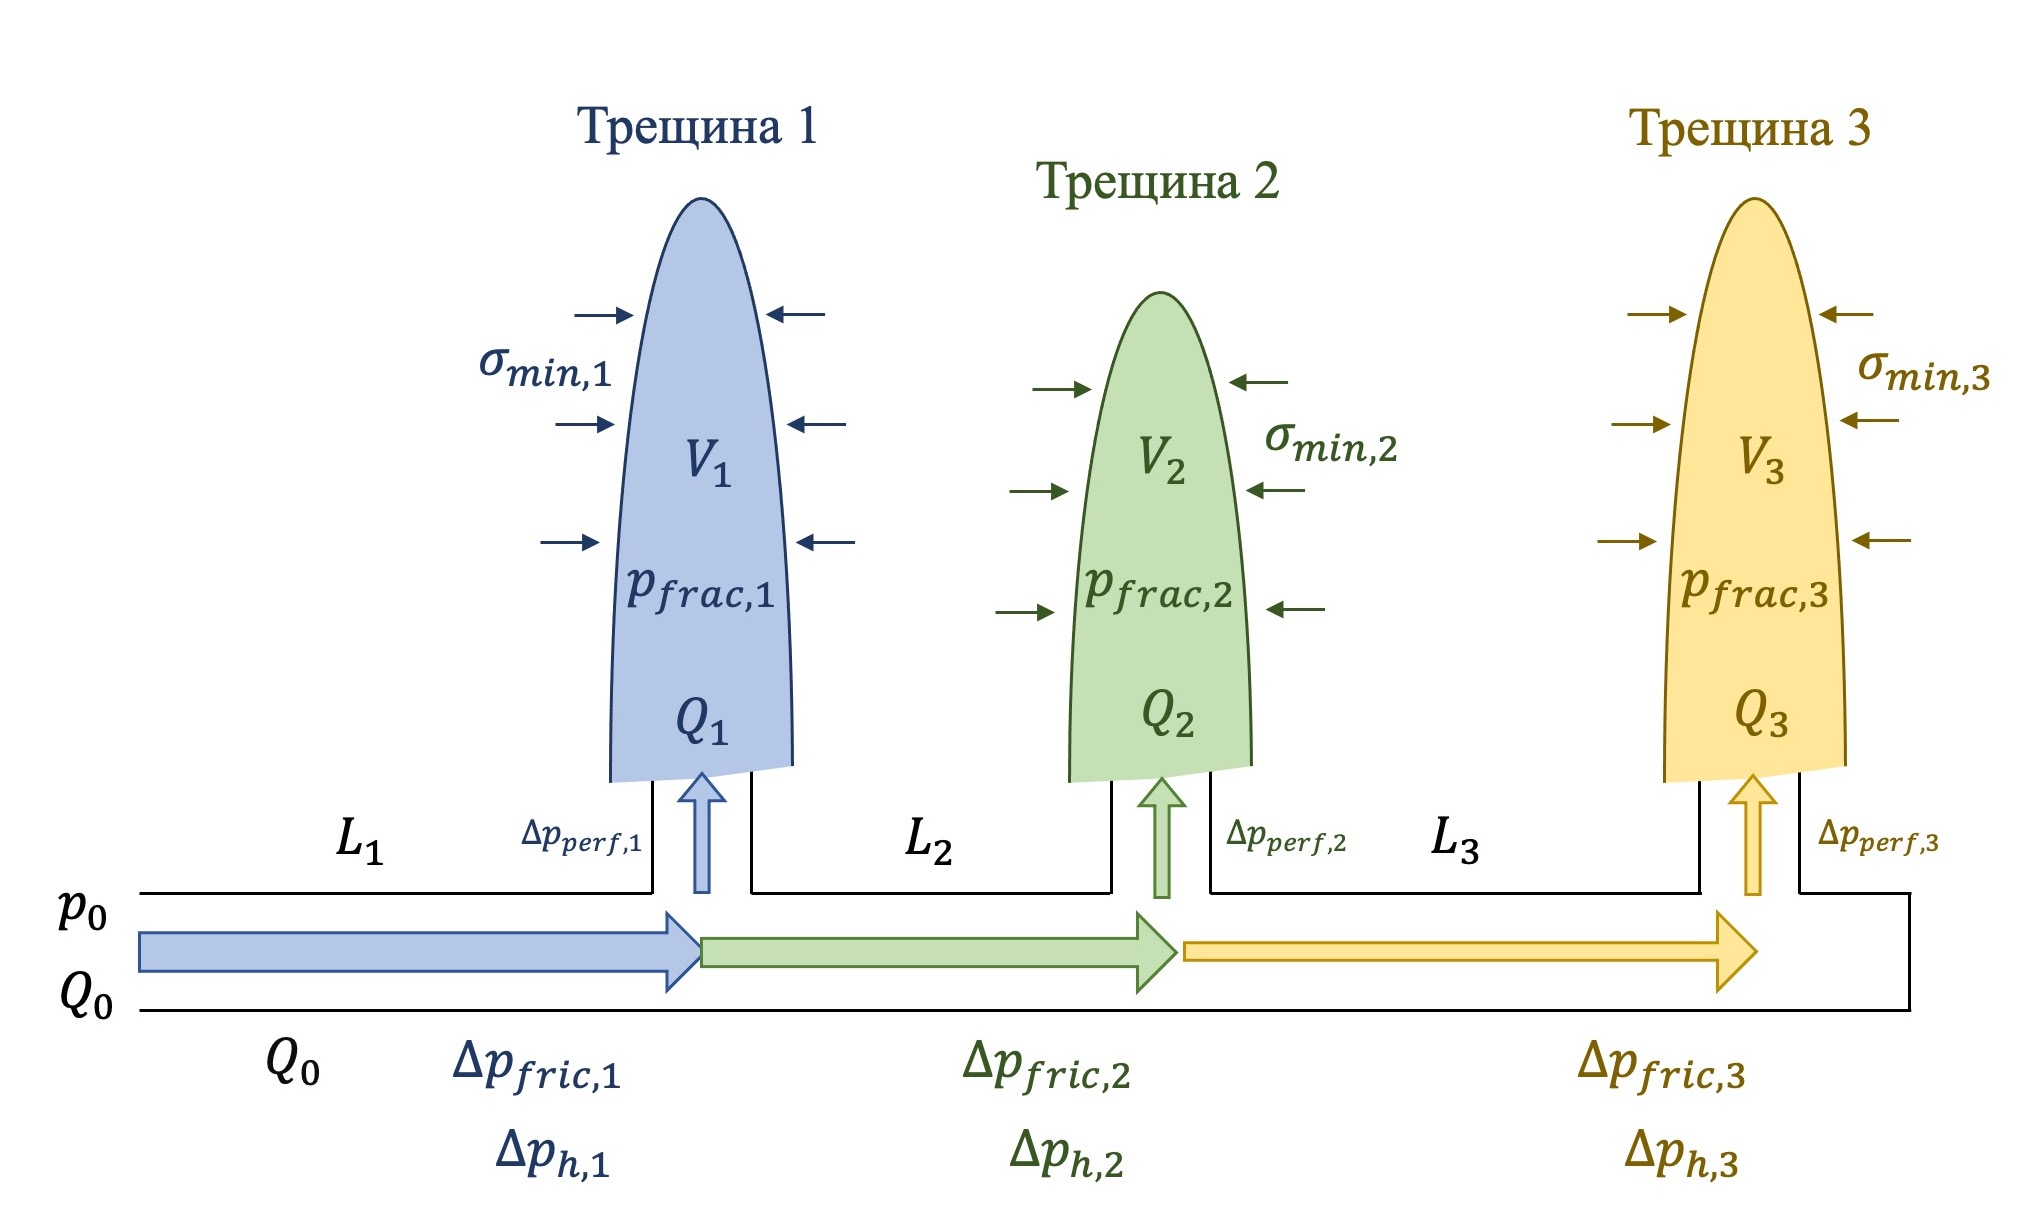
\includegraphics[width=10cm]{flow_distribution_scheme.jpg}
\end{textblock*}

\begin{textblock*}{4cm}(0cm,7.5cm)
$$Q_0=\sum\limits_{i=1}^{N}Q_i\,\,\,;$$
\end{textblock*}

\begin{textblock*}{10.5cm}(2.7cm,7.5cm)
$$p_0=\sigma_{\text{min},i}+p_{\text{net},i}+\Delta p_{\text{perf},i}-\sum_{j=1}^{i}{\Delta p_{h,\,j}}+\sum_{j=1}^{i}\Delta p_{\text{fric},\,j}$$
\end{textblock*}

\end{frame}


\begin{frame}
\frametitle{Формула Кёнинга}


\end{frame}


\begin{frame}
\frametitle{Использование полной производной полудлины трещины по времени}


\end{frame}



\end{document}
